\section{Algorytm genetyczny hybrydowy (memetyczny)}

\subsection{Wstęp}

Algorytmy memetyczne są pewnym ulepszeniem w stosunku do genetycznych. Stosowane są w nich dodatkowo algorytmy wyszukiwania lokalnego, które powinny zwiększać dokładność otrzymanych wyników.\\
Jeśli chodzi o implementację, uruchomienie algorytmu hybrydowego z wykorzystaniem pakietu \textit{GA} różni się od zwykłego genetycznego jedynie parametrem \textit{optim} ustawionym na \textit{TRUE}.

\subsubsection{Wyniki badań}

\begin{figure}[H]
	\centering
	\hspace*{-0.8in}
	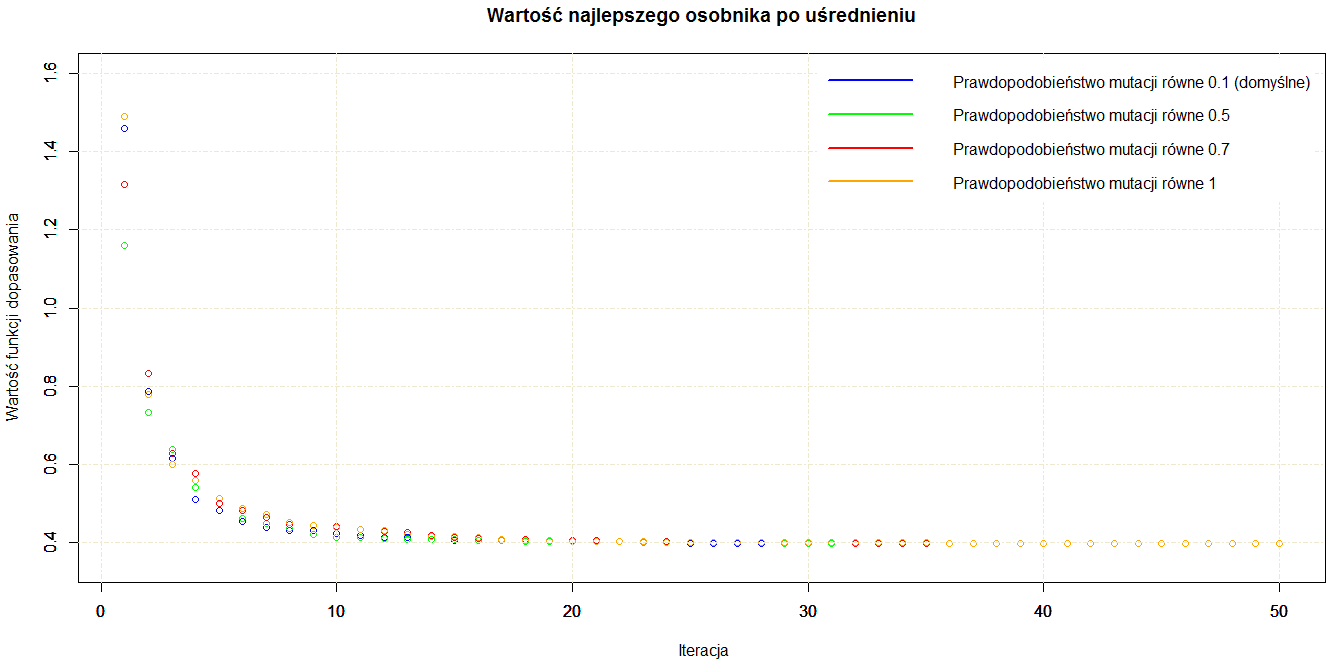
\includegraphics[scale = 0.5]{zad3_mut_max}
	\caption{Wartości najlepszych osobników dla różnych prawdopodobieństw mutacji}  
	\label{rys:zad3_mut_max} 
\end{figure}

\begin{figure}[H]
	\centering
	\hspace*{-0.8in}
	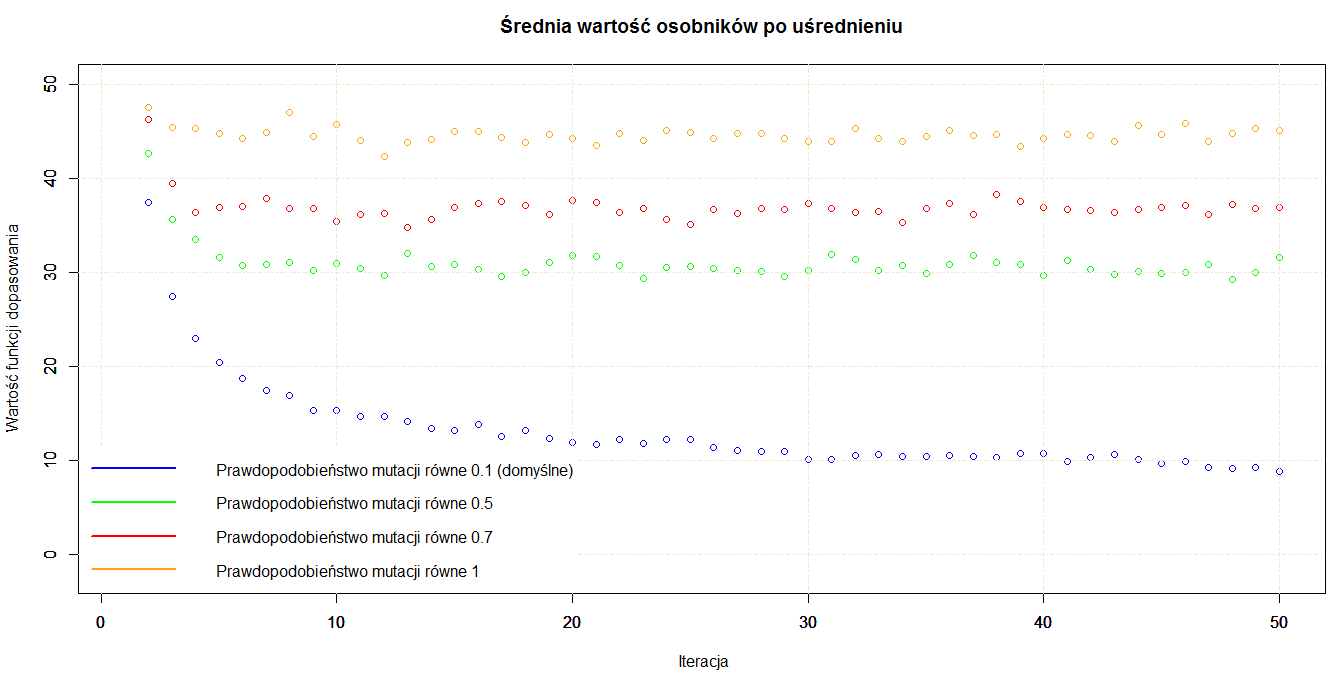
\includegraphics[scale = 0.5]{zad3_mut_mean}
	\caption{Wartości średnie osobników dla różnych prawdopodobieństw mutacji}  
	\label{rys:zad3_mut_mean} 
\end{figure}

\begin{figure}[H]
	\centering
	\hspace*{-0.8in}
	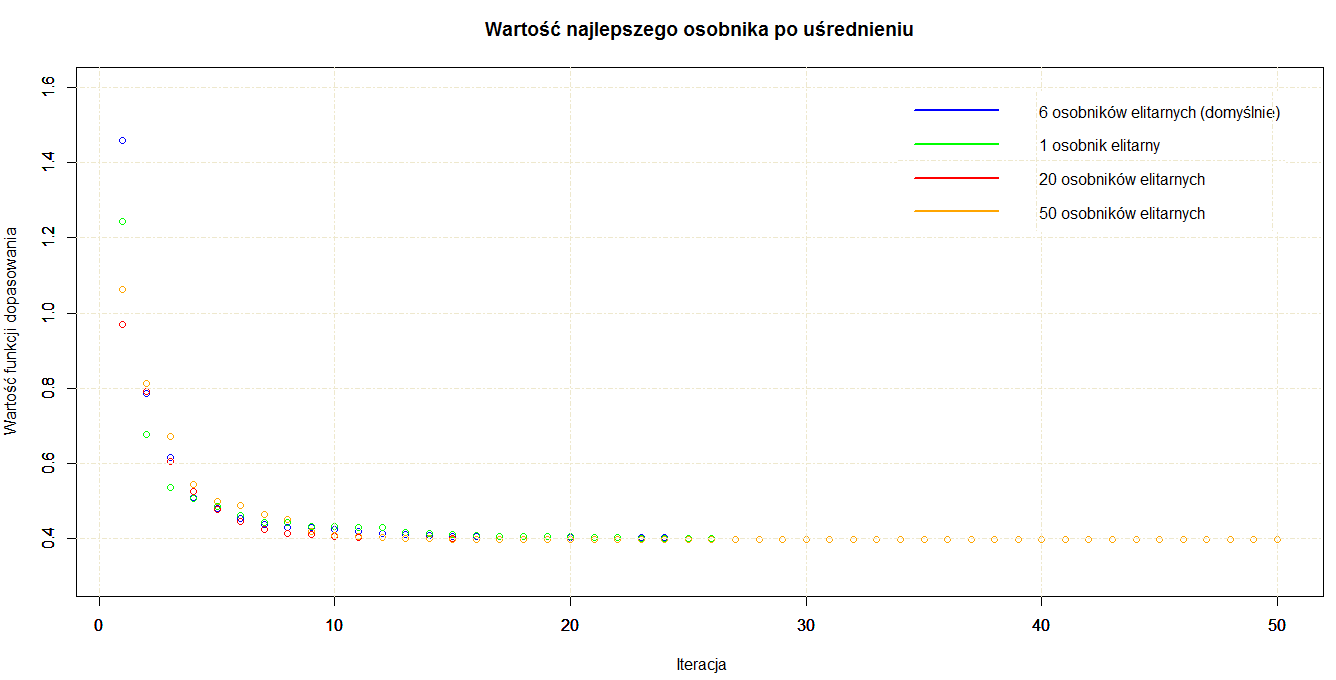
\includegraphics[scale = 0.49]{zad3_sel_max}
	\caption{Wartości najlepszych osobników dla różnej ilości osobników elitarnych}  
	\label{rys:zad3_sel_max} 
\end{figure}

\begin{figure}[H]
	\centering
	\hspace*{-0.8in}
	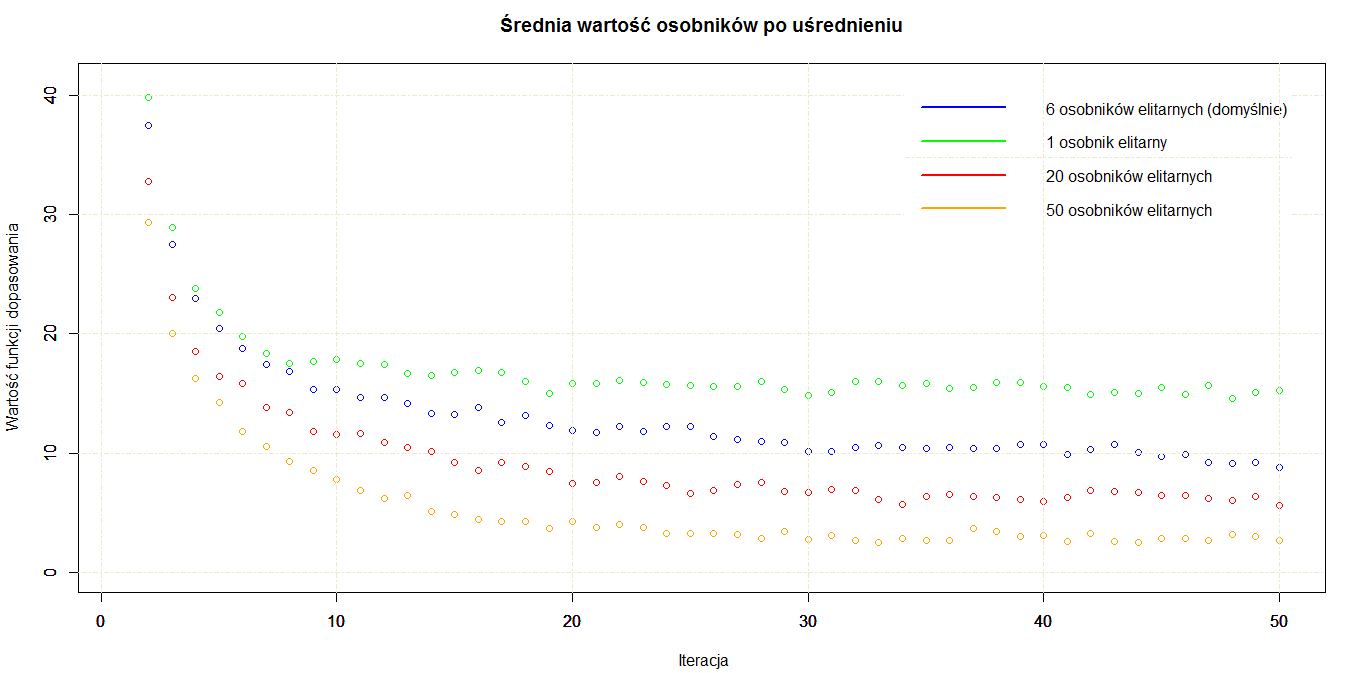
\includegraphics[scale = 0.45]{zad3_sel_mean}
	\caption{Wartości średnie osobników dla różnej ilości osobników elitarnych}  
	\label{rys:zad3_sel_mean} 
\end{figure}

\vline

\subsubsection{Wnioski}

\begin{table}[!h]
	\hspace*{-1.5in}
	\centering
	\caption{Wartości średnie i najlepsze osobnika dla różnych prawdopodobieństw mutacji}
	\label{mut_alg_hyb}
	\hspace*{-0.4in}
	\begin{tabular}{|c|c|c|c|c|}
		\hline
		\textbf{Prawdopodobieństwo mutacji} & \textbf{Wartość średnia} & \textbf{Najlepszy wynik} \\ \hline
		
		0.1 & 8.811131 & 0.398058 \\
		0.5 & 31.624510 & \textbf{{\color{green} 0.397912 }} \\
		0.7 & 36.915900 & 0.397930 \\
		1   & 45.09641 & 0.398302 \\ \hline      
	\end{tabular}
\end{table}


\begin{table}[!h]
	\hspace*{-1.5in}
	\centering
	\caption{Wartości średnie i najlepsze osobnika dla różnych ilości osobników elitarnych}
	\label{sel_alg_hyb}
	\hspace*{-0.4in}
	\begin{tabular}{|c|c|c|c|c|}
		\hline
		\textbf{Liczba osobników elitarnych} & \textbf{Wartość średnia} & \textbf{Najlepszy wynik} \\ \hline
		
		6  & 8.811131 & 0.398058 \\
		1  & 15.28275 & 0.398001 \\
		20 & 5.619913 & \textbf{{\color{green} 0.397887}} \\
		50 & 2.657782 & \textbf{{\color{green} 0.397887}} \\ \hline      
	\end{tabular}
\end{table}

W przypadku selekcji elitarnej udało się uzyskać rezultat identyczny (z dokładnością \mbox{do 0.000 001)} z podanym w dokumentacji minimum lokalnym funkcji \textit{branin}. Tym samym zostały potwierdzone założenia teoretyczne, jakoby algorytm hybrydowy miał polepszyć wyszukiwanie lokalnego extremum.